\chapter{PENDAHULUAN}

\section{Latar Belakang}

\noindent Indonesia merupakan negara maritim dengan luas laut dan perairan 62\% \parencite{inproc:wuryadani}. Potensi ini harus didukung berdasarkan prinsip \textit{Blue Economy}. \textit{Blue Economy} sendiri merupakan komponen penting dalam pengembangan keberlanjutan yang berfokus pada ekonomi maritim yang meliputi berbagai sektor seperti perikanan, akuakultur, dan transportasi maritim. Konsep \textit{Blue Economy} berkaitan erat dengan \textit{Sustainable Development Goal} ke 14 yang membahas mengenai pelestarian dan penggunaan lautan, laut, dan sumber daya laut secara berkelanjutan \parencite{misc:lse}. Menurut Departemen Perhubungan (2020), transportasi laut memegang peran strategis untuk mendorong pertumbuhan ekonomi di Indonesia. Salah satu bentuk untuk mendukung rencana jangka panjang ini adalah melalui upaya efisiensi penggunaan bahan bakar.

Efisiensi sendiri terbagi menjadi dua, yakni Efisiensi Teknologi dan Efisiensi Manajemen. Efisiensi Teknologi merujuk pada keterbaruan teknologi mesin yang mampu menghemat penggunaan bahan bakar dari waktu ke waktu. Sedangkan pada Efisiensi Manajemen memastikan bahwa bahan bakar sepenuhnya digunakan untuk mendukung operasi. Fokusan pada penelitian ini adalah Efisiensi Manajemen. Untuk itu, diperlukan sebuah teknologi untuk melakukan validasi data penggunaan bahan bakar yang dilaporkan dengan nilai aktual yang dihabiskan. 

Seiring dengan perkembangan teknologi komputer serta jangkauan konektivitas internet yang meluas, lahirlah sebuah teknologi bernama \textit{Internet of Things}. IoT atau \textit{Internet of Things} merupakan teknologi transformatif yang berpotensi merevolusi berbagai industri melalui kontrol dan pemantauan ekstensif secara jarak jauh \parencite{article:hercog}. Sejauh ini, IoT telah diterapkan di berbagai sektor seperti perumahan, pertanian, transportasi, dan lainnya. Kemampuan teknologi IoT dalam memberikan data secara jarak jauh membuka jalan bagi pelaku industri untuk merealisasi efisiensi bahan bakar pada transportasi laut. Hal ini senada dengan penelitian yang dilakukan \textcite{article:suciu}, yang menyatakan IoT memungkinkan integrasi mesin, sistem, dan proses untuk meningkatkan efisiensi operasional dan \textit{predictive maintenance}.

Langkah untuk melakukan efisiensi dengan kontrol melalui teknologi IoT juga dinilai tepat mengingat minyak fosil akan habis di tahun 2070 \parencite{misc:bp} sehingga pelaku industri tidak hanya menghemat biaya operasional, melainkan juga mendukung ekonomi serta menjaga lingkungan secara berkelanjutan. Salah satu dampak yang ditimbulkan dari belum diterapkannya teknologi ini adalah kurangnya kontrol yang mengakibatkan celah pada pelanggaran hukum. Pada tahun 2020 terdapat kasus penggelapan bahan bakar yang mencapai 2.5 ton liter \parencite{misc:aditya}, sehingga menimbulkan kerugian negara mencapai 710 juta rupiah. Hal ini dapat diatasi menggunakan sistem \textit{monitoring} berbasis IoT yang memungkinkan pemantauan konsumsi bahan bakar secara jarak jauh. Sistem \textit{monitoring} berbasis IoT merupakan suatu sistem yang menggunakan Internet of Things untuk memantau dan menyimpan data dari berbagai sensor.

PT Bisma Jaya merupakan perusahaan jasa transportasi laut yang berbasis di Balikpapan. Berdasarkan hasil diskusi dengan direktur operasional mitra, belum terdapat suatu alat yang memungkinkan manajemen untuk melakukan pemantauan kecepatan mesin serta bahan bakar kapal.  Saat ini, digunakan laporan harian dan bulanan sebagai acuan dalam mengestimasi jumlah bahan bakar yang diperlukan di bulan berikutnya. Pada akhirnya, mitra pernah cukup kesulitan memberikan penjelasan ketika terjadi ketidaksesuaian jumlah bahan bakar di tangki kapal ketika dilakukan validasi sebelum pengisian. Oleh karenanya, dibutuhkan sistem \textit{monitoring} berbasis IoT yang memungkinkan kontrol dan penyimpanan data secara historis. Lebih lanjut, sistem ini akan digunakan mitra untuk memantau kecepatan mesin agar sesuai dengan ketentuan yang berlaku, memastikan penggunaan bahan bakar termanfaatkan dengan maksimal serta meningkatkan rasa percaya antara manajemen dan pekerja di lapangan. 

Untuk merealisasi penelitian ini dibutuhkan lintas disiplin ilmu, yakni elektronika dan komputer. Oleh karena itu, dibutuhkan suatu metode pengembangan sistem yang lebih menekankan kolaborasi serta komunikasi yang baik. Terdapat metode \textit{Waterfall}, yang merupakan proses desain sekuensial yang digunakan dalam proyek pengembangan perangkat lunak. Ini mengikuti perkembangan linier melalui fase yang berbeda, termasuk pengumpulan dan analisis kebutuhan, desain, pengkodean, pengujian, dan pemeliharaan \parencite{article:abbas}. Metode ini, mengasumsikan kebutuhan telah final di awal proyek, serta tiap fase harus diselesaikan terlebih dahlu sebelum lanjut ke fase berikutnya. Oleh karenanya, metode ini tidak cocok untuk diterapkan pada sistem yang memiliki kebutuhan yang dinamis. Sehingga, penggunaan metode \textit{Waterfall} dirasa kurang cocok dalam pengembangan Sistem \textit{Monitoring} berbasis IoT dikarenakan sulitnya untuk mengatur perubahan dan beradaptasi pada kebutuhan yang berkembang.

\textit{Agile} merupakan pendekatan yang secara efektif dapat beradaptasi dengan kebutuhan yang berubah-ubah, yang mana ini sulit untuk diatur pada model \textit{Waterfall}. Salah satu metode yang populer adalah Scrum. Scrum merupakan metodologi yang berfokus pada pengembangan berulang dan bertahap, fleksibilitas, dan perbaikan terus menerus. Metodologi ini sangat cocok untuk pengembangan proyek skala masif dengan personel pengembang yang banyak. 

Lalu terdapat metode \textit{Extreme Programming} (XP), sebuah metode agile yang menekankan pada kolaborasi, adaptasi, dan pengembangan iteratif \parencite{article:matharu}. \textit{Extreme Programming} metode yang ideal untuk digunakan tim skala kecil menengah dalam pengembangkan perangkat lunak dengan cepat serta fleksibel dalam menghadapi perubahan. Salah satu prinsip dari metode ini adalah keterlibatan pelanggan \parencite{article:matharu}. Hal ini memastikan perangkat lunak memenuhi kebutuhan pelanggan dan mengurangi risiko pengembangan fitur yang tidak diperlukan.

Berdasarkan pertimbangan pilihan metode yang sudah dilakukan, metode yang paling cocok untuk diterapkan pada studi kasus penelitian ini adalah metode \textit{Extreme Programming} (XP) karena dari perusahaan membutuhkan sistem yang dapat dengan cepat diimplementasikan tanpa harus melalui proses dokumentasi yang banyak. Metode ini cocok untuk pengembangan sistem dengan tim yang sedikit dan dalam kurun waktu yang relatif singkat, serta bersifat fleksibel terhadap perubahan dikarenakan adanya kemungkinan perubahan kebutuhan terkait fitur-fitur yang ada pada sistem. 

Diharapkan dengan adanya penelitian ini, sistem \textit{monitoring} pada mesin diesel yang dikembangkan dapat membantu PT Bisma Jaya khususnya direktur operasional dalam melakukan pemantauan penggunaan bahan bakar serta menjaga efektivitas armada kapal yang sedang beroperasi yang mulanya melalui laporan harian/bulanan menjadi sistem yang dapat memberi informasi secara real time.



\section{Rumusan Masalah}

\noindent Berdasarkan latar belakang dari penelitian, didapatkan rumusan masalah sebagai berikut.

\begin{enumerate}
    \item Bagaimana sistem monitoring dirancang menggunakan metode Extreme Programming?
    \item Bagaimana sistem monitoring dikembangan menggunakan metode Extreme Programming?
\end{enumerate}

\section{Tujuan}

\noindent Tujuan dari penelitian ini adalah sebagai berikut.

\begin{enumerate}
    \item Untuk merancang sistem monitoring menggunakan metode Extreme Programming.
    \item Untuk mengembangkan sistem monitoring menggunakan metode Extreme Programming.
\end{enumerate}

\section{Manfaat}

\noindent Manfaat yang didapatkan pada penelitian ini adalah sebagai berikut.

\begin{enumerate}
    \item Membantu perusahaan dalam melakukan pengawasan dan kontrol konsumsi bahan bakar armada kapal selama operasi.
    \item Membantu perusahaan dalam memastikan efektivitas operasi  
\end{enumerate}


\section{Batasan Penelitian}

\noindent Batasan penelitian ini adalah sebagai berikut.

\begin{enumerate}
    \item Fokus utama pada penelitian ini adalah pengembangan sistem web
    \item Pada penelitian ini diterapkan 3 layer arsitektur IoT teratas: App Layer, Data Processing Layer, dan Network Layer (Penjelasan lebih detail terdapat di Bab Metode)
    \item Sistem Monitoring berbasis IoT dikembangkan menggunakan framework NextJS, Django, dan MySQL sebagai Database Management Systems (DBMS)
\end{enumerate}
\section{Kerangka Pemikiran Penelitian}

\noindent Berikut kerangka pikiran pada penelitian ini.

\begin{figure}[ht]
    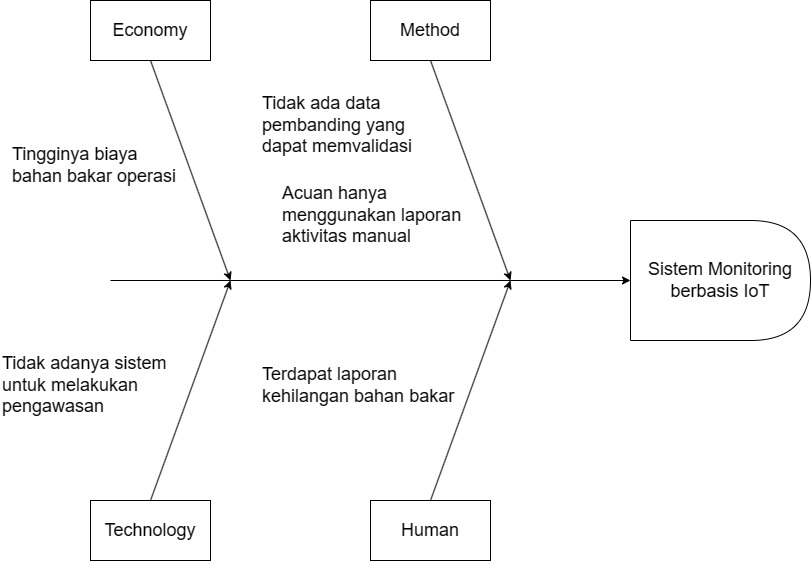
\includegraphics[width=1\linewidth, center]{images/pendahuluan/fig-framework-penelitian.jpg}
    \caption{Kerangka Penelitian}
    \label{fig:thinking-framework}
\end{figure}

\noindent Gambar 1.1  merupakan kerangka pemikiran penelitian yang bertujuan untuk memberikan gambaran mengenai urgensi implementasi sistem monitoring berbasis \textit{Internet of Things (IoT)} di PT Bisma Jaya. Perusahaan ini dihadapkan pada masalah utama berupa tingginya pengeluaran untuk bahan bakar selama operasionalnya, yang dipengaruhi oleh sejumlah permasalahan dalam aspek-aspek ekonomi, metode, teknologi, dan manusia.

Kategori ekonomi, pengguna jasa perusahaan telah mengalami situasi di mana mereka melaporkan adanya kejadian kehilangan bahan bakar. Sebelum armada kapal mengisi ulang bahan bakarnya, operator fuel management pengguna jasa akan melakukan pengukuran yang dikenal dengan istilah "sounding." Hasil dari pengukuran ini akan dibandingkan dengan laporan harian yang disusun oleh tim operasional kapal. Apabila ditemukan selisih sebesar lebih dari 100 liter, operator fuel management akan melaporkan indikasi kehilangan yang dapat mengakibatkan dikenakan denda.

Kategori metode, perusahaan selama ini mengandalkan laporan bulanan yang dibuat tim operasional kapal. Hanya saja, tidak ada data faktual yang dapat dijadikan pembanding terhadap laporan yang dibuat. Selain itu, laporan tersebut baru diterima setiap akhir bulan, sehingga perusahaan tidak memiliki data apapun hingga mendapat temuan dari pihak pengguna.

Kategori metode, perusahaan selama ini mengandalkan laporan bulanan yang dibuat tim operasional kapal. Hanya saja, tidak ada data faktual yang dapat dijadikan pembanding terhadap laporan yang dibuat. Selain itu, laporan tersebut baru diterima setiap akhir bulan, sehingga perusahaan tidak memiliki data apapun hingga mendapat temuan dari pihak pengguna.

Kategori manusia, laporan harian secara rutin dibuat setiap malamnya oleh tim operasional kapal. Selama operasi, mereka menjaga catatan aktivitas dalam sebuah jurnal yang mencatat waktu perjalanan dan berhenti kapal. Namun, terdapat kekurangan dalam pencatatan yaitu ketidakadanya pencatatan jumlah jam operasi pada tiap kategori operasi tertentu. Akibatnya, ketika mereka membuat laporan, nilai running hour untuk tiap kategori operasi hanya dapat diestimasikan saja, yang bisa berpotensi mengakibatkan ketidakakuratan data dan informasi yang vital dalam perhitungan konsumsi bahan bakar. Informasi lebih lanjut mengenai kategori operasi dapat dilihat pada bab metode.

Secara garis besar, didapatkan inti permasalahan yang terjadi di PT Bisma Jaya adalah tingginya biaya bahan bakar operasional pada sejumlah kapal, sehingga pada penelitian ini akan dikembangkan sistem monitoring mesin diesel yang akan membantu perusahaan dalam melakukan pemantauan jumlah bahan bakar selama operasi. 

% \blindtext 
% \cite{book:darma}